\vspace*{2em}
\phantomsection
\section*{Definition}
\addcontentsline{toc}{section}{Definition}
We say that a vertex $V$ in a graph $G$ with $C$
connected components is an \textit{articulation point} if its removal increases the number of connected components of $G$.
In other words, let $C'$ be the number of connected components after removing vertex $V$, if $C' > C$ then $V$ is an \textit{articulation point}.

\begin{figure}[H]
  \centering
  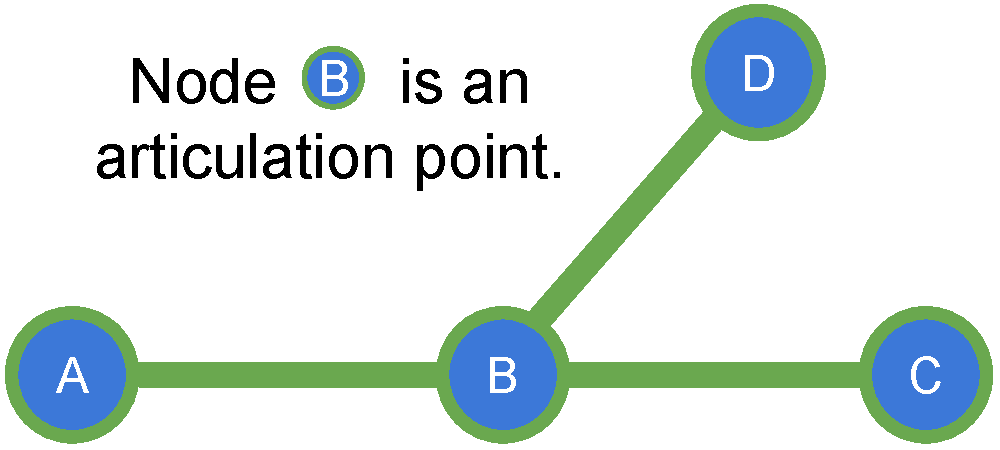
\includegraphics[width=0.35\textwidth]{"Images/Graph Theory/Articulation Points And Bridges/g1.pdf"}
  \caption{}
  \label{fig:apb_g1}
\end{figure}

\phantomsection
\section*{Naive Approach}
\addcontentsline{toc}{section}{Naive Approach}

\begin{figure}[thp]
  \centering
  \begin{minipage}[c]{0.9\textwidth}
    \begin{minted}[bgcolor=lightgray]{ruby}
for every vertex V in the graph G do
    Remove V from G
    if the number of connected components increases then
        V is an articulation point
    Add V back to G
      \end{minted}
  \end{minipage}
\end{figure}

The complexity of counting the number of \textit{connected components} is $O(V + E)$ therefore,
the total complexity of this naive approach is $O(V * (V + E))$.

\phantomsection
\section*{Tarjan's Approach}
\addcontentsline{toc}{section}{Tarjan's Approach}

First, we need to know that an \textit{ancestor} of some node $V$ is a node $A$ that was discoverd
before $V$ in a DFS traversal. i.e. In the graph of figure \ref{fig:apb_g1} shown above, if we start
our DFS from $A$ and follow the path to $C$ through $B$ ($A \rightarrow B \rightarrow C$), then $A$
is an ancestor of $B$ and $C$ in this spanning tree generated from the DFS traversal.\\

\begin{figure}[H]
  \centering
  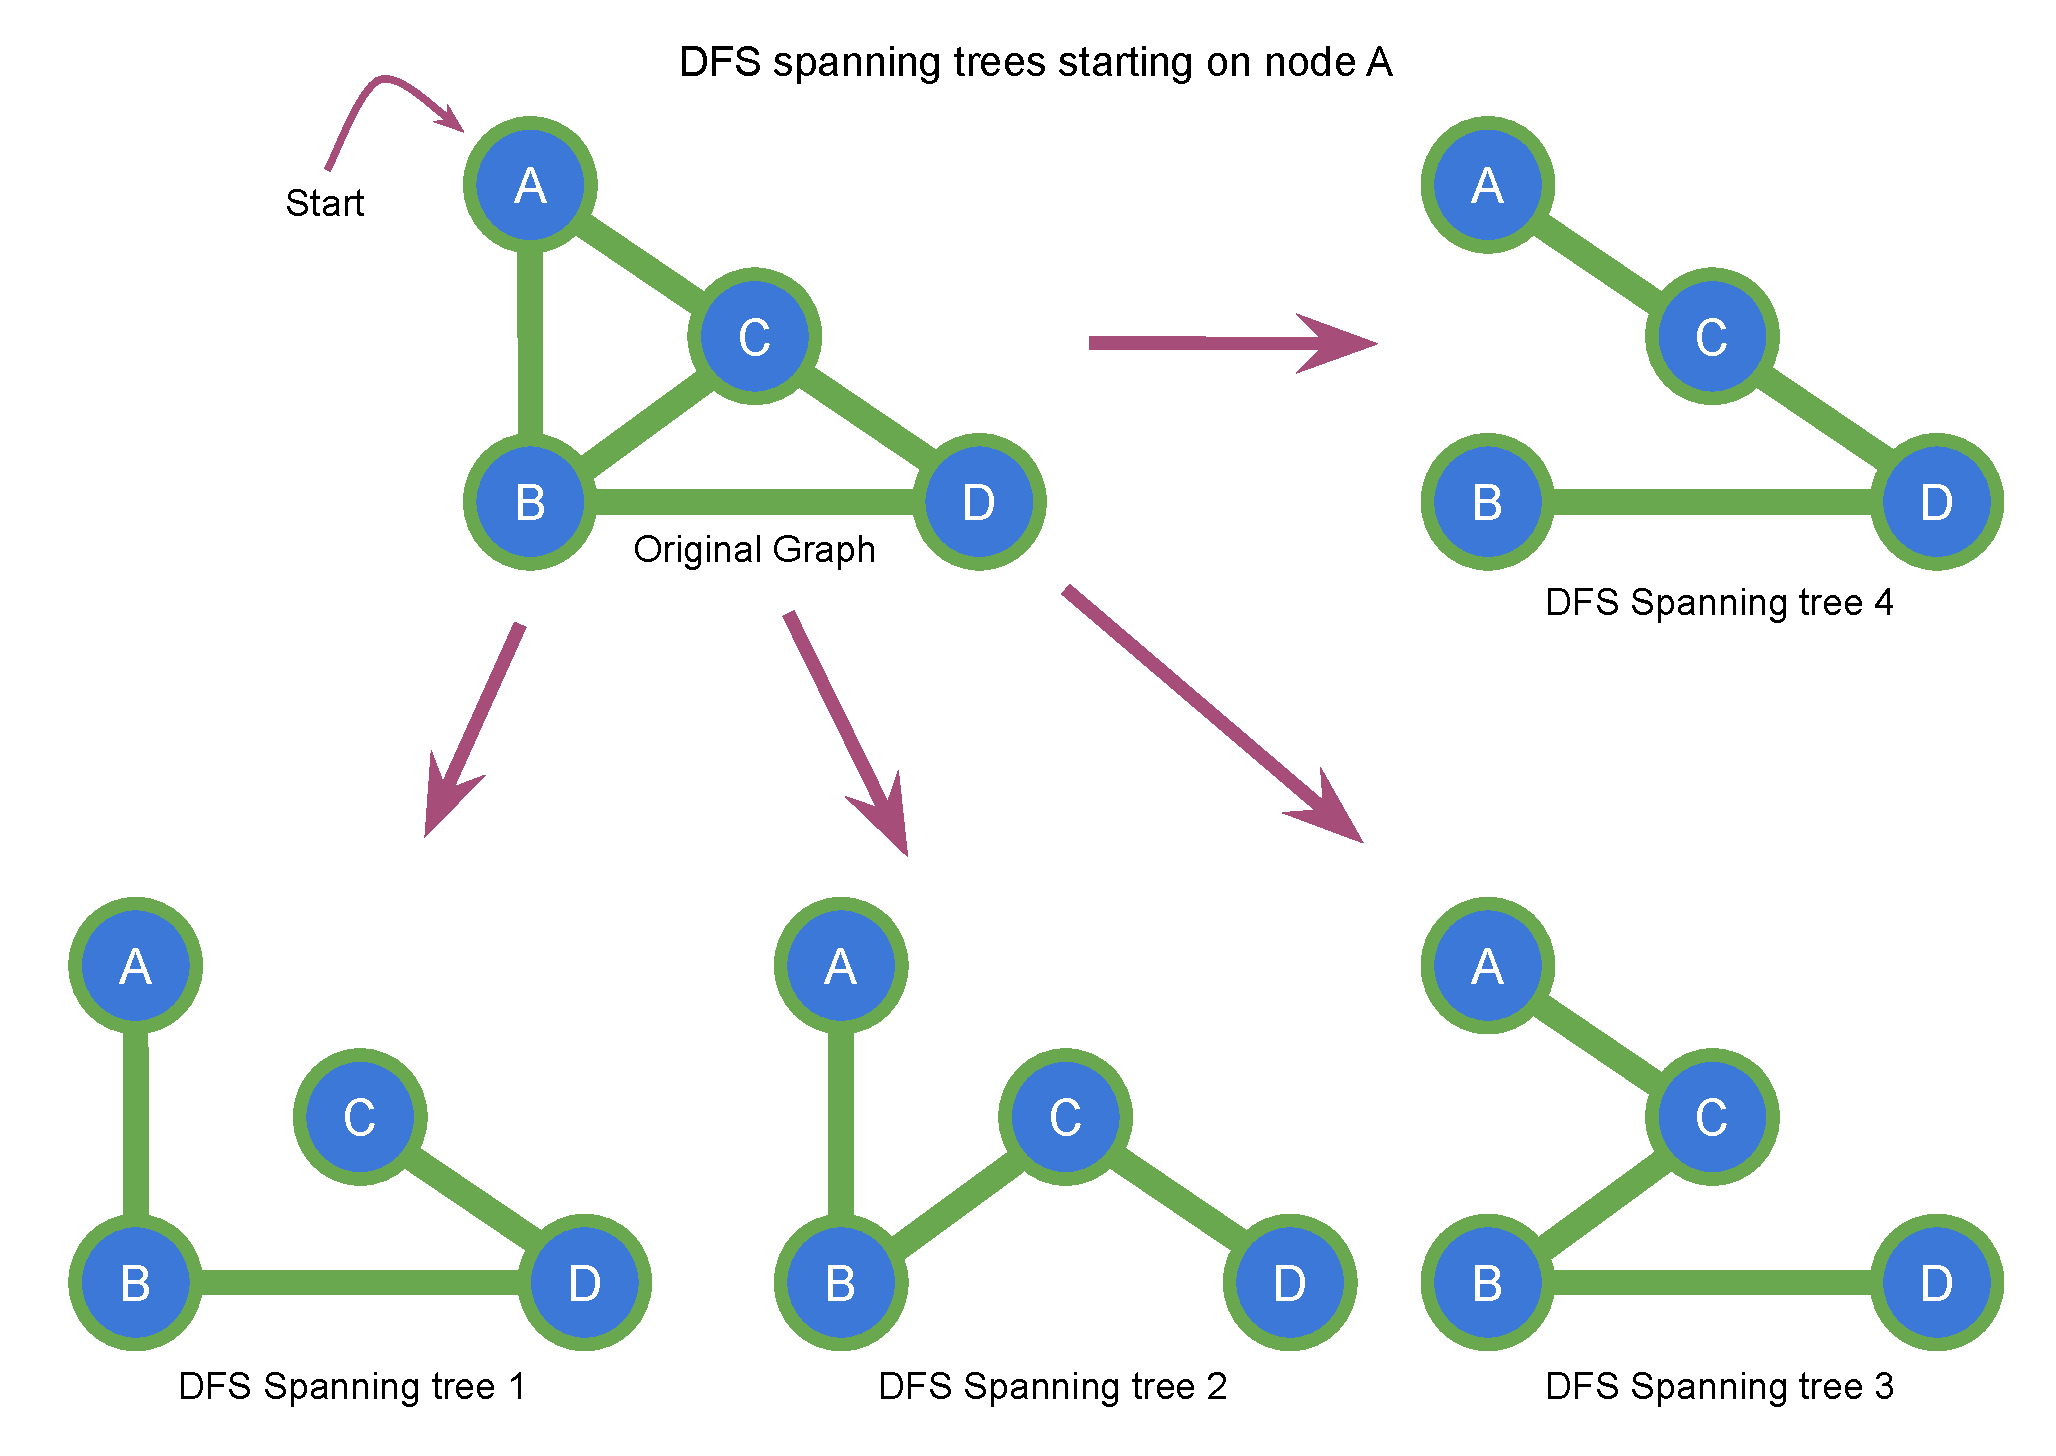
\includegraphics[width=0.7\textwidth]{"Images/Graph Theory/Articulation Points And Bridges/g2.pdf"}
  \caption{Example of DFS spanning trees of a graph}
  \label{fig:apb_g2}
\end{figure}


Now that we know the definition of \textit{ancestor} let's dive into the main idea.

\phantomsection
\subsection*{Idea}
\addcontentsline{toc}{subsection}{Idea}

Let's say there is a node $V$ in some graph $G$ that can be reached by a node $U$ through some
intermediate nodes (maybe non intermediate nodes) following some DFS traversal, if $V$ can also be
reached by $A$ = ''ancestor of $U$'' without passing through $U$ then, $U$ is NOT an articulation point
because it means that if we remove $U$ from $G$ we can still reach $V$ from $A$, hence, the number of
\textit{connected components} will remain the same. Hence, we can conclude that the only 2 conditions for
$U$ to be an \textit{articulation point} are:

\begin{enumerate}
  \item If all paths from $A$ to $V$ require $U$ to be in the graph.
  \item If $U$ is the root of the DFS traversal with at least 2 children subgraphs disconnected from each other.
\end{enumerate}

\noindent
Then we can break condition \#1 into 2 subconditions:

\begin{itemize}
  \item[\bullet] $U$ is an \textit{articulation point} if all paths from an ancestor of $U$ to $V$
        require $U$ to be in the graph.
        \begin{figure}[H]
          \centering
          
\includegraphics[width=0.5\textwidth]{"Images/Graph Theory/Articulation Points And Bridges/g9.pdf"}
          \caption{}
          \label{fig:apb_g3}
        \end{figure}
  \item[\bullet] $U$ is an \textit{articulation point} if it is the root of some cycle in the DFS traversal.
        \begin{figure}[H]
          \centering
          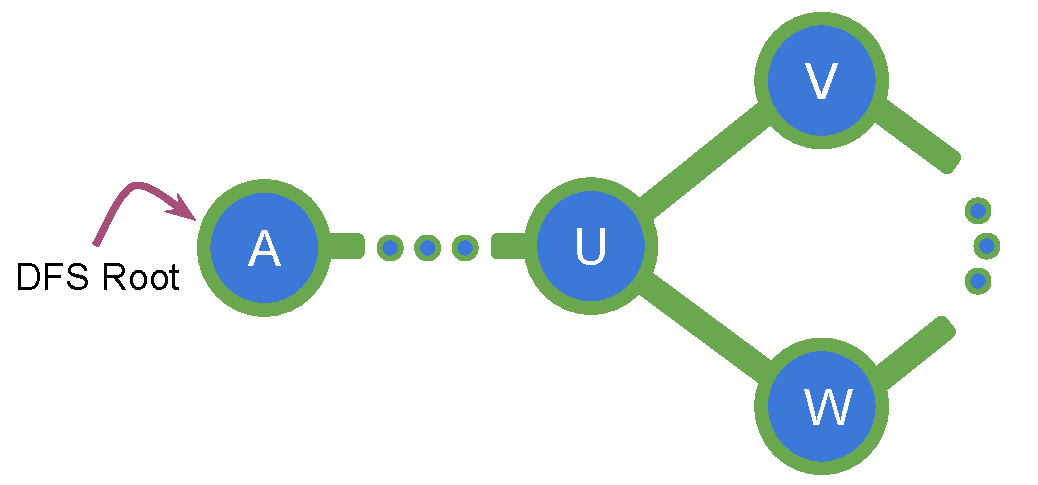
\includegraphics[width=0.5\textwidth]{"Images/Graph Theory/Articulation Points And Bridges/g8.pdf"}
          \caption{}
          \label{fig:apb_g3}
        \end{figure}
\end{itemize}